En el proceso de Scrum, las reuniones son de suma importancia y en cada paso en el proceso existen tipos de reuniones con sus propias características. Las reuniones principales que destaca Scrum son: Planificación de sprint, reunión diaria, revisión del sprint y reunión retrospectiva del sprint. En la \textbf{Figura~\ref{fig: reunionesScrum}} se ve el ciclo de Scrum desde el punto de vista de las reuniones.

\begin{figure}[ht!]
    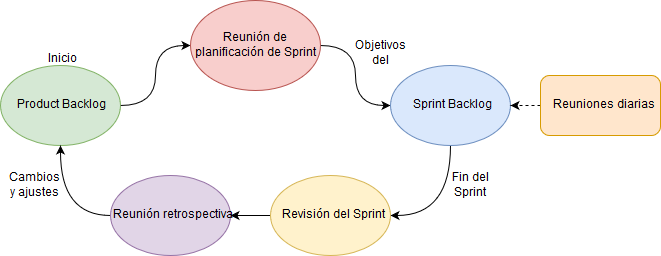
\includegraphics[width=\textwidth]{Imagenes/Reuniones_Scrum.jpg}
    \caption{\label{fig: reunionesScrum} Reuniones en el Proceso de Scrum.}
\end{figure}

\begin{itemize}
    \item   \begin{description}
                \item[Planificación del sprint: ] Los sprints tienen como objetivo convertir el back\-log del sprint en un incremento. Es por ello que antes de comenzar cada uno de ellos, se deben reunir el PO, el scrum master y el equipo para definir en cuál funcionalidad se debe trabajar, asumiendo que los objetivos no van a cambiar durante este sprint. Para ello se debe tener en cuenta la estimación de esfuerzo dedicado a trabajos de soporte o de preparación del ambiente que requiere el proyecto, los requerimientos de recursos de infraestructura o logístico (máquinas, redes, pizarra, etc.), entre otras.
                
                Esta reunión consta de dos partes; la primera, el equipo junto con el product owner seleccionan la lista de requisitos que se convertirán en el incremento del siguiente sprint según la prioridad hecha por los participantes de la reunión. Mientras que en la segunda parte, se debe planificar el trabajo del sprint, definiendo las tareas que se realizarán en el backlog de este último.

            \end{description}

    \item   \begin{description}
                \item[Reunión diaria:] juntas de corto periodo (por lo general quince minutos) las cuales se realizan a diario por el equipo de Scrum, en donde todos los miembros del equipo se deben plantear y responder las siguientes tres preguntas:  
                
                \begin{itemize}
                    \item ¿Qué hiciste desde la última reunión?

                    \item ¿Cuáles obstáculos encontraste? 

                    \item ¿Qué esperas lograr para la siguiente reunión del equipo?
                \end{itemize}

                Durante cada reunión, los integrantes deben reportar sus avances y/o problemas enfrentados durante el trabajo realizado hasta ese momento, por lo que la confianza es fundamental dentro del equipo en esta fase. Cabe señalar que con esta acción de reportar problemas, se espera que los integrantes tengan una reacción de apoyo (referente al problema y con motivo de solucionarlo) y retroalimentación. Esto voto de confianza permite que cada integrante sepa en que está trabajando cada uno.
            \end{description}
    
    \item   \begin{description}
                \item[Revisión del sprint: ] En esta reunión se inspecciona el trabajo realizado durante el sprint. Para ello, los equipos de trabajo presentan el incremento que se construyó, el cual es supervisado por el PO y los stakeholders. Por otro lado, deben indicar qué resultó bien y mal del incremento, las observaciones que surgieron durante éste y se realiza una demostración del producto que todos pueden ver. Aquí nuevamente se destaca la importancia de la confianza entre el equipo y el SM. Por último, basándose en la inspección se toman decisiones sobre qué realizar en el siguiente sprint, sin descartar la realización de adaptaciones al proyecto. 
        
            \end{description}

    \item   \begin{description}
                \item[Reunión retrospectiva del del sprint: ] proceso cuyo objetivo principal es discutir acerca de los pro y contras del sprint finalizado y determinar si se requiere modificar algo para una iteración mejor con mayor productividad. Los participantes de esta reunión hacen referencia en el cómo se construyó el incremento anterior y cualquier cosa que afecte al equipo, ya sea procesos, prácticas, comunicación, entorno, artefactos y herramientas. Este tipo de reunión es de gran importancia ya que permite mejorar al equipo de trabajo durante cada etapa del proyecto. Por otra parte, los que pueden participar en esta reunión son el equipo, el PO y el SM, teniendo todo el derecho de opinar abiertamente sobre el trabajo realizado.

            \end{description}
\end{itemize}
